% Posterior factorization
\section{}
% --- From Bayes' rule to the ELBO (variational lower bound) ---

\paragraph{Goal.}
We would like to infer the latent quantities $(z,\theta)$ given the data $(X,Y)$ and hyperparameters $\psi$,
i.e., we want the posterior distribution $p(z,\theta\mid X,Y,\psi)$.

\paragraph{Bayes' rule and the hard part.}
By Bayes' rule,
\begin{equation}\label{eq:posterior_bayes}
p(z,\theta \mid X,Y,\psi)
=\frac{p(Y \mid X,z,\theta,\psi)\,p(z,\theta \mid \psi)}{p(Y \mid X,\psi)}.
\end{equation}
The numerator (likelihood $\times$ prior) is typically easy to evaluate. Note that here we have assumed
that the prior $p(z,\theta\mid \psi)$ does not depend on $X$, $p(z,\theta\mid \psi) = p(z,\theta\mid \psi, X)$; if it does, the following derivation still holds with $p(z,\theta\mid \psi) = p(z,\theta\mid \psi, X)$.
The difficulty is the denominator $p(Y\mid X,\psi)$, which is the \emph{normalizing constant}
(often called the \emph{evidence} or \emph{marginal likelihood}) that makes the posterior integrate to one.

\paragraph{Rewriting the evidence as an integral.}
We can express the evidence by integrating out the latent variables:
\begin{align}
\log p(Y \mid X,\psi)
&= \log \iint p(Y,z,\theta \mid X,\psi)\,dz\,d\theta. \label{eq:evidence_integral}
\end{align}
For notational convenience, define the joint latent vector $\lambda := (z,\theta)$, so the same quantity becomes
\begin{align}
\log p(Y \mid X,\psi)
&= \log \int p(Y,\lambda \mid X,\psi)\,d\lambda. \label{eq:evidence_lambda}
\end{align}
This step makes explicit what we are trying to compute: the evidence is an integral over latent variables.
In most interesting models this integral is intractable, which motivates an approximation.

\paragraph{Introducing a variational distribution.}
We now introduce an arbitrary density $q(\lambda)$ (the \emph{variational distribution}) and multiply and divide by it:
\begin{align}
\log p(Y \mid X,\psi)
&= \log \int q(\lambda)\,\frac{p(Y,\lambda \mid X,\psi)}{q(\lambda)}\,d\lambda. \label{eq:insert_q}
\end{align}

\paragraph{Jensen's inequality and the ELBO.}
Applying Jensen's inequality to $\log\big(\mathbb{E}_q[\cdot]\big)$ yields a lower bound:
\begin{align}
\log p(Y \mid X,\psi)
&\ge \int q(\lambda)\,\log\frac{p(Y,\lambda \mid X,\psi)}{q(\lambda)}\,d\lambda. \label{eq:jensen_elbo}
\end{align}
Next we factor the joint distribution as
$p(Y,\lambda\mid X,\psi)=p(Y\mid X,\psi,\lambda)\,p(\lambda\mid X,\psi)$, giving
\begin{align}
\int q(\lambda)\,\log\frac{p(Y,\lambda \mid X,\psi)}{q(\lambda)}\,d\lambda
&= \int q(\lambda)\,\log\frac{p(Y\mid X,\psi,\lambda)\,p(\lambda\mid X,\psi)}{q(\lambda)}\,d\lambda \label{eq:factor_joint}\\
&= \int q(\lambda)\,\log p(Y\mid X,\psi,\lambda)\,d\lambda
\;-\;\mathrm{KL}\!\left(q(\lambda)\,\|\,p(\lambda\mid X,\psi)\right). \label{eq:elbo_kl_prior}
\end{align}
The first term is an expectation of the log-likelihood under $q$.
The second term is a Kullback--Leibler divergence that regularizes $q$ towards the prior
(or towards $p(\lambda\mid X,\psi)$ if the prior depends on $X$).

\paragraph{ELBO + KL-to-posterior decomposition (tightness).}
Define the evidence lower bound (ELBO) as
\begin{equation}\label{eq:elbo_def}
\mathcal{L}(q)
:= \int q(\lambda)\,\log\frac{p(Y,\lambda\mid X,\psi)}{q(\lambda)}\,d\lambda.
\end{equation}
Then one can show the exact identity
\begin{equation}\label{eq:elbo_plus_kl}
\log p(Y\mid X,\psi)
= \mathcal{L}(q) + \mathrm{KL}\!\left(q(\lambda)\,\|\,p(\lambda\mid X,Y,\psi)\right).
\end{equation}
Because KL divergences are nonnegative, $\mathcal{L}(q)$ is indeed a lower bound on $\log p(Y\mid X,\psi)$.
Moreover, the bound becomes tight exactly when
\begin{equation}\label{eq:q_is_posterior}
q(\lambda)=p(\lambda\mid X,Y,\psi),
\end{equation}
in which case $\mathrm{KL}(q\,\|\,p(\lambda\mid X,Y,\psi))=0$ and $\mathcal{L}(q)=\log p(Y\mid X,\psi)$.

% ------------------------------------------------------------
% Appendix: Deriving the (negative) ELBO loss for the SeqGPLVM
% ------------------------------------------------------------

\subsection{From Bayes' rule to an optimizable loss (ELBO)}

\paragraph{Key idea.}
Our inferential target is the posterior over latent quantities, which 
include the latent variables and parameters, (and possibly hyperparameters):
\(
p(\boldsymbol{\lambda}\mid \mathbf{X},\mathbf{Y},\boldsymbol{\psi})
\),
where \(\boldsymbol{\psi}\) denotes (fixed) hyperparameters. Bayes' rule gives
\begin{equation}
p(\boldsymbol{\lambda}\mid \mathbf{X},\mathbf{Y},\boldsymbol{\psi})
=
\frac{p(\mathbf{Y}\mid \mathbf{X},\boldsymbol{\lambda},\boldsymbol{\psi})\,p(\boldsymbol{\lambda}\mid \mathbf{X},\boldsymbol{\psi})}
     {p(\mathbf{Y}\mid \mathbf{X},\boldsymbol{\psi})},
\label{eq:bayes-posterior}
\end{equation}
where the denominator
\(
p(\mathbf{Y}\mid \mathbf{X},\boldsymbol{\psi})
\)
(the \emph{marginal likelihood} / \emph{evidence}) is the normalizing constant. In latent-variable models this term is typically intractable; introducing a tractable variational density \(q(\boldsymbol{\lambda})\) yields a lower bound on \(\log p(\mathbf{Y}\mid\mathbf{X},\boldsymbol{\psi})\). Crucially, the gap between this bound and the true log-evidence is a KL divergence to the true posterior, so maximizing the bound pushes \(q(\boldsymbol{\lambda})\) towards \(p(\boldsymbol{\lambda}\mid \mathbf{X},\mathbf{Y},\boldsymbol{\psi})\).

\paragraph{Variational lower bound and KL-to-posterior decomposition.}
Let \(\boldsymbol{\lambda}\) collect all latent variables and parameters to be inferred. The marginal likelihood can be written as
\begin{align}
\log p(\mathbf{Y}\mid \mathbf{X},\boldsymbol{\psi})
&= \log \int p(\mathbf{Y},\boldsymbol{\lambda}\mid \mathbf{X},\boldsymbol{\psi})\,\mathrm{d}\boldsymbol{\lambda}
\nonumber\\
&= \log \int q(\boldsymbol{\lambda})\,
\frac{p(\mathbf{Y},\boldsymbol{\lambda}\mid \mathbf{X},\boldsymbol{\psi})}{q(\boldsymbol{\lambda})}\,
\mathrm{d}\boldsymbol{\lambda}
\nonumber\\
&\ge \int q(\boldsymbol{\lambda})
\log\frac{p(\mathbf{Y},\boldsymbol{\lambda}\mid \mathbf{X},\boldsymbol{\psi})}{q(\boldsymbol{\lambda})}\,
\mathrm{d}\boldsymbol{\lambda}
\;=:\; \mathcal{L}(q),
\label{eq:elbo-def}
\end{align}
where the inequality is Jensen's inequality.
Using Bayes' rule,
\(
p(\boldsymbol{\lambda}\mid \mathbf{X},\mathbf{Y},\boldsymbol{\psi})
=
p(\mathbf{Y},\boldsymbol{\lambda}\mid \mathbf{X},\boldsymbol{\psi})/p(\mathbf{Y}\mid \mathbf{X},\boldsymbol{\psi})
\),
one obtains the standard identity
\begin{align}
\mathrm{KL}\!\left(q(\boldsymbol{\lambda})\,\|\,p(\boldsymbol{\lambda}\mid \mathbf{X},\mathbf{Y},\boldsymbol{\psi})\right)
&=
\int q(\boldsymbol{\lambda})
\log\frac{q(\boldsymbol{\lambda})}{p(\boldsymbol{\lambda}\mid \mathbf{X},\mathbf{Y},\boldsymbol{\psi})}\,
\mathrm{d}\boldsymbol{\lambda}
\nonumber\\
&=
\log p(\mathbf{Y}\mid \mathbf{X},\boldsymbol{\psi})
-\int q(\boldsymbol{\lambda})
\log\frac{p(\mathbf{Y},\boldsymbol{\lambda}\mid \mathbf{X},\boldsymbol{\psi})}{q(\boldsymbol{\lambda})}\,
\mathrm{d}\boldsymbol{\lambda}
\nonumber\\
&= \log p(\mathbf{Y}\mid \mathbf{X},\boldsymbol{\psi}) - \mathcal{L}(q).
\label{eq:logp-elbo-kl}
\end{align}
Equivalently,
\begin{equation}
\log p(\mathbf{Y}\mid \mathbf{X},\boldsymbol{\psi})
=
\mathcal{L}(q)
+
\mathrm{KL}\!\left(q(\boldsymbol{\lambda})\,\|\,p(\boldsymbol{\lambda}\mid \mathbf{X},\mathbf{Y},\boldsymbol{\psi})\right),
\label{eq:logp-decomp}
\end{equation}
so maximizing \(\mathcal{L}(q)\) w.r.t.\ \(q\) minimizes the KL divergence to the true posterior (and equality holds iff \(q(\boldsymbol{\lambda}) = p(\boldsymbol{\lambda}\mid \mathbf{X},\mathbf{Y},\boldsymbol{\psi})\)). 
This is true since the lhs of \eqref{eq:logp-decomp} does not depend on \(q\).

\subsection{SeqGPLVM: inducing variables and the resulting ELBO}

\paragraph{Inducing variables and GP conditionals.}
For each time step \(t\in\{1,\dots,T\}\), let \(\mathbf{f}_t\in\mathbb{R}^{N}\) denote latent GP function values at the \(N\) observed inputs and \(\mathbf{u}_t\in\mathbb{R}^{M}\) the inducing variables at inducing inputs \(\mathbf{M}_t\) (collecting \(M\) inducing locations). With kernel hyperparameters \(\boldsymbol{\psi}_t\), define kernel matrices
\(
\mathbf{K}^{(t)}_{NN}, \mathbf{K}^{(t)}_{NM}, \mathbf{K}^{(t)}_{MN}, \mathbf{K}^{(t)}_{MM}
\)
computed from the (time-\(t\)) GP inputs (in the GPLVM these inputs may involve \(\mathbf{X}\) and the latent \(\mathbf{z}\); we suppress this dependence in the conditioning to keep notation light).
The sparse GP prior uses
\begin{align}
p(\mathbf{u}_t\mid \boldsymbol{\psi}_t) &= \mathcal{N}\!\left(\mathbf{0},\mathbf{K}^{(t)}_{MM}\right),
\\
p(\mathbf{f}_t\mid \mathbf{u}_t,\boldsymbol{\psi}_t)
&=\mathcal{N}\!\left(
\mathbf{K}^{(t)}_{NM}(\mathbf{K}^{(t)}_{MM})^{-1}\mathbf{u}_t,\;
\mathbf{K}^{(t)}_{NN}-\mathbf{K}^{(t)}_{NM}(\mathbf{K}^{(t)}_{MM})^{-1}\mathbf{K}^{(t)}_{MN}
\right).
\label{eq:gp-conditional}
\end{align}

\paragraph{Latent variables and variational family.}
Let \(\mathbf{z}\in\mathbb{R}^{d}\) denote the (global) latent variable(s) with prior
\begin{equation}
p(\mathbf{z})=\mathcal{N}(\mathbf{0},\mathbf{I}).
\label{eq:z-prior}
\end{equation}
Collect all latents as
\(
\boldsymbol{\lambda} := (\mathbf{z},\mathbf{f}_{1:T},\mathbf{u}_{1:T})
\),
where \(\mathbf{f}_{1:T}:=(\mathbf{f}_1,\dots,\mathbf{f}_T)\) and similarly for \(\mathbf{u}_{1:T}\).
We use the standard sparse variational GP factorization
\begin{equation}
q(\boldsymbol{\lambda})
=
q(\mathbf{z})\prod_{t=1}^{T} q(\mathbf{u}_t)\,p(\mathbf{f}_t\mid \mathbf{u}_t,\boldsymbol{\psi}_t),
\qquad
q(\mathbf{z})=\mathcal{N}(\mathbf{m}_z,\mathbf{S}_z),
\quad
q(\mathbf{u}_t)=\mathcal{N}(\mathbf{m}_{u_t},\mathbf{S}_{u_t}).
\label{eq:q-factorization}
\end{equation}

\paragraph{Sequential likelihood factorization.}
Assume a time-factorized observation model (conditional on the latent state):
\begin{equation}
p(\mathbf{Y}\mid \mathbf{X},\mathbf{z},\mathbf{f}_{1:T},\boldsymbol{\psi})
=
\prod_{t=1}^{T}
p\!\left(\mathbf{y}_t \mid \mathbf{X}_t,\mathbf{Y}_{1:t-1},\mathbf{z},\mathbf{f}_t,\boldsymbol{\psi}_t\right),
\label{eq:seq-likelihood}
\end{equation}
where \(\mathbf{y}_t\in\mathbb{R}^{N}\) is the vector of observations at time \(t\) and \(\mathbf{Y}_{1:t-1}\) collects past observations.

\paragraph{ELBO for the SeqGPLVM.}
Plugging \eqref{eq:q-factorization} and \eqref{eq:seq-likelihood} into the generic ELBO \eqref{eq:elbo-def} yields
\begin{align}
\mathcal{L}(q)
&=
\mathbb{E}_{q(\boldsymbol{\lambda})}
\left[
\log p(\mathbf{Y}\mid \mathbf{X},\boldsymbol{\lambda},\boldsymbol{\psi})
\right]
-
\mathrm{KL}\!\left(q(\boldsymbol{\lambda})\,\|\,p(\boldsymbol{\lambda}\mid \mathbf{X},\boldsymbol{\psi})\right)
\nonumber\\
&=
\sum_{t=1}^{T}
\mathbb{E}_{q(\mathbf{z})\,q(\mathbf{u}_t)\,p(\mathbf{f}_t\mid \mathbf{u}_t,\boldsymbol{\psi}_t)}
\left[
\log p\!\left(\mathbf{y}_t \mid \mathbf{X}_t,\mathbf{Y}_{1:t-1},\mathbf{z},\mathbf{f}_t,\boldsymbol{\psi}_t\right)
\right]
\nonumber\\
&\quad
-\sum_{t=1}^{T}\mathrm{KL}\!\left(q(\mathbf{u}_t)\,\|\,p(\mathbf{u}_t\mid \boldsymbol{\psi}_t)\right)
-\mathrm{KL}\!\left(q(\mathbf{z})\,\|\,p(\mathbf{z})\right).
\label{eq:seqgplvm-elbo}
\end{align}
The corresponding training loss is the negative ELBO,
\begin{equation}
\mathcal{J}_{\text{VI}}(\boldsymbol{\psi})
:=
-\mathcal{L}(q),
\label{eq:neg-elbo-loss}
\end{equation}
optionally optimized jointly over the variational parameters \(\{(\mathbf{m}_z,\mathbf{S}_z),(\mathbf{m}_{u_t},\mathbf{S}_{u_t})\}_{t=1}^T\) and hyperparameters \(\boldsymbol{\psi}\).

\paragraph{Optional: hyperprior regularization.}
If a hyperprior \(p(\boldsymbol{\psi})\) is used, then (up to an additive constant) one targets
\begin{equation}
\log p(\boldsymbol{\psi}\mid \mathbf{X},\mathbf{Y})
\propto
\log p(\mathbf{Y}\mid \mathbf{X},\boldsymbol{\psi}) + \log p(\boldsymbol{\psi})
\;\approx\;
\mathcal{L}(q) + \log p(\boldsymbol{\psi}),
\label{eq:elbo-plus-hyperprior}
\end{equation}
and in the time-separable case \( \log p(\boldsymbol{\psi}) = \sum_{t=1}^{T}\log p(\boldsymbol{\psi}_t)\).

\newpage
\begin{landscape}
\begin{figure}[p]
  \centering
  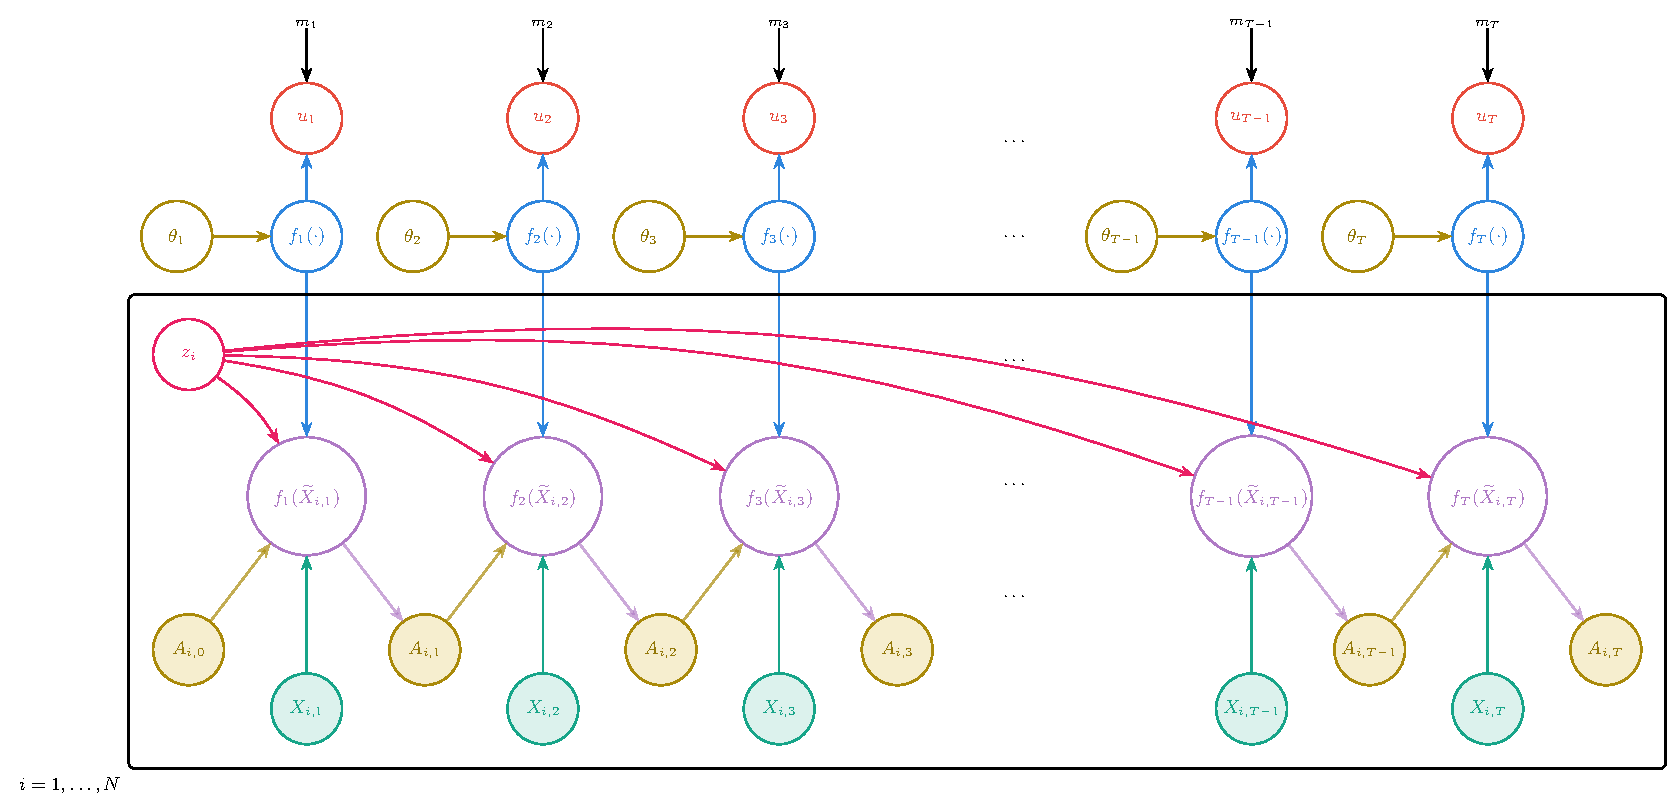
\includegraphics[width=\textwidth]{figures/build/fit_seqgplvm_dag.pdf}
  \caption{...}
  \label{fig:seqdecon}
\end{figure}
\end{landscape}

